\documentclass{article}
\usepackage{amsmath}
\usepackage{amsthm}
\usepackage{amsfonts}
\usepackage{mathtools}
\usepackage{graphicx}
\title{MATH 620: Homework 2}
\author{Fernando}
\date{October 10, 2023}
\begin{document}
\maketitle
\section{Problem 1}
\subsection{Part a}
We want to write $D=\{x_0+y: y\in V\}$ (where V is a linear subspace).
In this case we can take $x_0=3x+2$ and $V=\{\phi\in X:
\phi(0)=\frac{\partial\phi}{\partial x}(1)=0\}$. It
is easy to see that $V$ is a linear subspace because it is closed under adition
and scalar product. Also the boundary conditions are satisfied so indeed we can
write $D$ in this way.
\subsection{Part b}
Take $\phi_1,\phi_2\in D$ we have to prove that:
$(1-\alpha)\phi_1+\alpha \phi_2 \in D,\forall \alpha \in [0,1]$.
This is clearly in $C^k([0,1])$ but also:
\[
\left((1-\alpha)\phi_1+\alpha\phi_2\right)(0)
=\left((1-\alpha)2+\alpha2\right)=2,
\]
and
\[
\left[\frac{\partial}{\partial x}\left((1-\alpha)\phi_1+\alpha \phi_2\right)\right](1)= 
\left((1-\alpha)\frac{\partial \phi_1}{\partial x}+\alpha\frac{\partial
\phi_2}{\partial x}\right)(1) = (1-\alpha)3+\alpha 3=3.
\]
So $D$ is convex.
\subsection{Part c}
$D'(x_0)$ is defined as
\[
	\{v\in X: x_0 +v \in D\},
\]
so in this case by definition:
\[
	D'=V=\{\phi\in X:
\phi(0)=\frac{\partial\phi}{\partial x}(1)=0\}.
\]
\section{Problem 2}
\subsection{Part a}
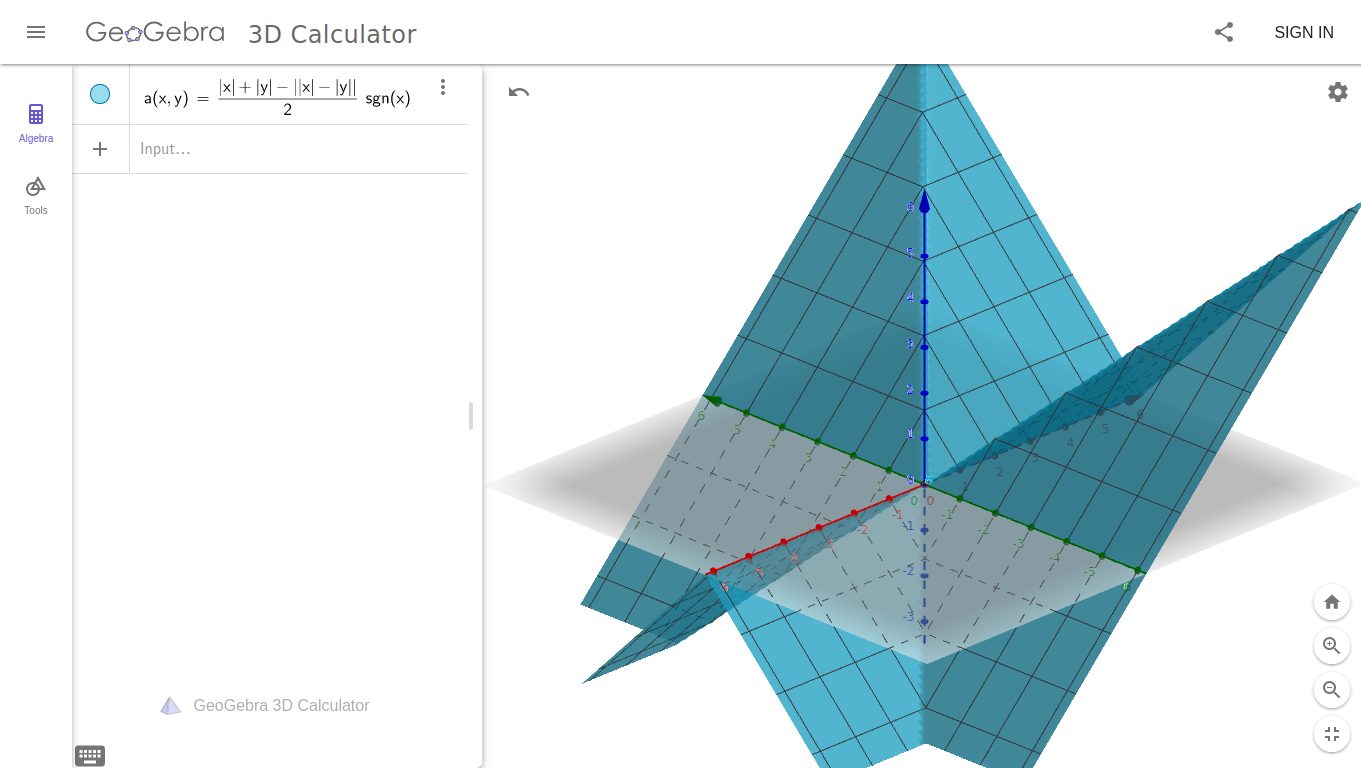
\includegraphics[width=\textwidth]{minsign.png}
In the image we can see that along the $x$ axis (red) the function is constant
and equal to 0. Same for the $y$ axis (green). So clearly the directional
derivative in the $x$ or $y$ direction at 0 will be 0, i.e. $\nabla f(0) =0$.

To see that this is not true for all directions we can take $x=y$ and we get
$f(x,y)=|x|\text{sign}(x)=x$ so the directional derivative of $f$ at 0 in the
direction of the vector $(1,1)$ is 1.
\subsection{Part b}
In this case the function is not $C^1$ so its change along a
certain direction cannot always be expressed in terms of the
gradient. This means that the strategy of looking for minimizers by setting the
gradient to 0 only works when the function we are dealing with is $C^1$.
\section{Problem 3}
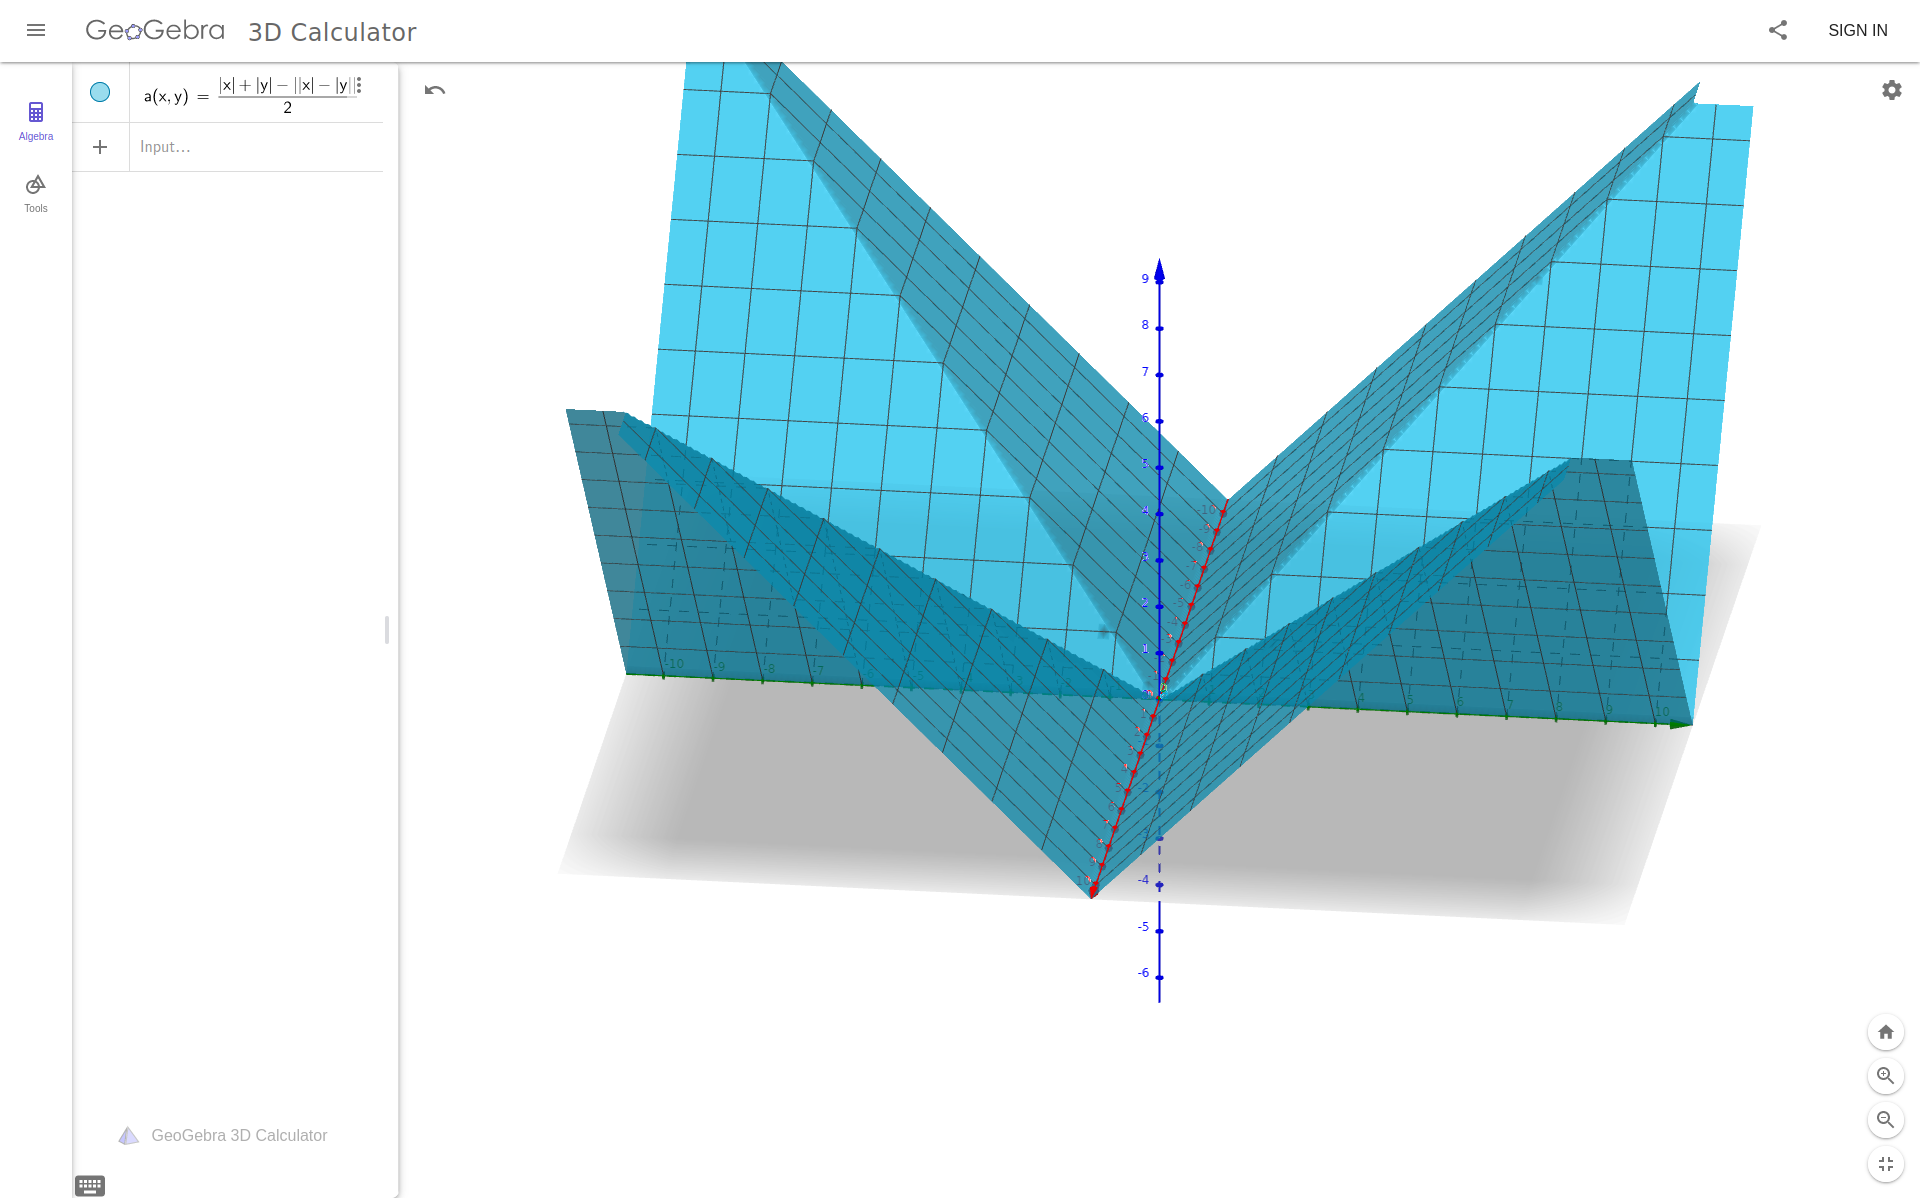
\includegraphics[width=\textwidth]{min.png}
Let's prove that $\nabla f(0)=0$.

That is $\frac{\partial f}{\partial x}(0)=\frac{\partial f}{\partial y}(0)=0$.
Which in this case is easy to see because $f(x,0)=f(0,y)=0$, which implies that
$\nabla f(0)=0$.

To prove that $f$ does not have a Gateaux derivative for all $v$ we can choose
$x=0$ and $v=(1,1)$ then $Df((0,0);(1,1))$ is by definition:
\begin{align*}
\lim_{\tau \to 0} \frac{f((0,0)+\tau(1,1))-f((0,0))}{\tau}
&= \lim_{\tau \to 0} \frac{f((\tau,\tau))-0}{\tau}\\
&=\lim_{\tau \to 0} \frac{|\tau|}{\tau}.
\end{align*}
Which does not exists, so $Df((0,0);(1,1))$ is not defined.
\end{document}
